\chapter{Marco Metodológico}

    En el presente capítulo se describe la metodología usada para el desarrollo del proyecto así como sus componentes, los actores que participaron y los roles que cumplieron en el desarrollo del mismo.

    Para \textit{HxPlus Ocupacional} fue seleccionado Scrum como metodología de desarrollo a seguir. Y aunque no está estipulado por la metodología, se llevó a cabo el diagrama de casos de uso visualización más completa del sistema.
    
    Scrum es una metodología de gestión de proyectos ágil que utiliza uno o más equipos de trabajo, de a lo sumo 7 personas, en iteraciones de tiempo fijo, llamados \textit{Sprints}, para la entrega de tareas o avances en el proyecto que sean funcionales y probados
    \footnote{Con información de \citeauthor{scrum-guia}\cite{scrum-guia}, \citeauthor{scrum-primer}\cite{scrum-primer} y \citeauthor{scrum-agile}\cite{scrum-agile}}.    
    
    Los equipos apuntan siempre a conseguir avances limpios, probados y aceptados de manera que puedan ser puestos en producción inmediatamente.
    
%    Scrum se divide en Roles, Eventos y Artefactos tal como se describe a continuación:

    \section{Roles}
        
        \subsection{Product Owner}
        \label{product-owner}
        
        Este rol representa la voz del cliente en la gestión del proyecto. Debe velar por la realización del proyecto desde la perspectiva del negocio. Se encarga de escribir las historias de usuario, las prioriza y las anexa al ``Product Balcklog" (o también Lista del Producto).
        
        El Dueño de Producto es la única persona responsable de gestionar la Lista del Producto. La gestión de dicha lista, según expresa \citeauthor{scrum-guia}\cite{scrum-guia}, consiste en:
        
        \begin{itemize}
            \item Expresar claramente los elementos de la Lista del Producto.
            \item Ordenar los elementos en la Lista del Producto para alcanzar los objetivos y misiones de la mejor manera posible.
            \item Optimizar el valor del trabajo desempeñado por el Equipo de Desarrollo.
            \item Asegurar que la Lista del Producto es visible, transparente y clara para todos, y que muestra aquello en lo que el equipo trabajará a continuación.
            \item Asegurar que el Equipo de Desarrollo entiende los elementos de la Lista del Producto al nivel necesario.
        \end{itemize}
               
        Para el presente proyecto se designó al ingeniero Juan Albarrán como Product Owner siendo el mejor representante de los intereses de Soluciones Globinsoft S.A. y estando él familiarizado tanto con los procesos de negocio como con el equipo de desarrollo y el proceso de desarrollo mismo.
        
        \subsection{Scrum Master}
        \label{scrum-master}
        
        Es el responsable de llevar el procedimiento de gestión del proyecto según los lineamientos de Scrum. Sirve de asesoría entre invloucrados y comprometidos en materia de organización y distribución de la información. Él dirige las reuniones y vela por su cumplimiento según las reglas de procedimiento de Scrum.
        
        \citeauthor{scrum-guia}\cite{scrum-guia} clasifica los servicios del Scrum Master en tres categorías:
        \begin{enumerate}
            \item Servicio al dueño del producto
            \begin{itemize}
                \item Asesoramiento para la gestión eficiente de la Lista del Producto.
                \item Asesoramiento para la planificación del producto.
            \end{itemize}
            
            \item Servicio al equipo de desarrollo
            \begin{itemize}
                \item Apoyar en la organización del equipo.
                \item Eliminar los impedimientos y dificultades que limiten el progreso del equipo.
                \item Facilitar la organización de los eventos de Scrum según sea requerido.
                \item Guiar al equipo en entornos donde Scrum no haya sido del todo adoptado.
                \item Apoyar al equipo en dudas que surjan respecto a los eventos y artefactos de Scrum.
            \end{itemize}
            \item Servicio a la organización
            \begin{itemize}
                \item Liderar la adopción de Scrum como metodología de desarrollo.
                \item Asesorar a los empleados en el uso de Scrum y sus procedimientos.
            \end{itemize}
        \end{enumerate}
        
       Por su experiencia en previos proyectos, entre ellos \textit{HxPlus} (antecedente de \textit{HxPlus Ocupacional}) y su amplio conocimiento en el negocio, se le delegó también el puesto de ``Scrum Master" en el presente proyecto al ingeniero Juan Albarrán.
        
        \subsection{Development Team}
        \label{development-team}
        
        Es el conjunto de personas dedicadas a construir el producto indicado por el dueño del producto. Se requieren que sean grupos lo suficientemente pequeños como para fomentar un alto nivel de independencia y autoorganización pero, a su vez, lo suficientemente grandes como para poder presentar avances significativos en cada Sprint y que potencialmente, estos avances, puedan ser puestos en producción.
        
        Equipos pequeños, de menos de tres personas, reduce la productividad global y reduce los posibles avances en el producto. También podrían presentar limitaciones en cuando a las habilidades de los integrantes, lo cual resultaría convirtiéndose en impedimentos en el desarrollo.
        
        Por otro lado, equipos muy grandes, de más de nueve miembros requiere demasiada coordinación entre los miembros lo cual podría significar una menor eficiciencia y mayor trabajo para la organización de los avances. En otras palabras, se perdería agilidad tratando de organizar un equipo semejante.
        
        Idealmente un equipo de desarrollo varía entre tres y siete personas. Esto mantiene un equilibrio saludable entre la cantidad de trabajo que pueden manejar y la capacidad de autoorganización del equipo.
        
        El equipo debe ser multifuncional, debe tener las capacidades necesarias para desarrollar el producto y poder apoyarse entre sí para compensar los puntos débiles de cada individuo.
        
        No existen roles dentro del equipo de desarrollo. A pesar que uno podría desempeñarse mejor en un área de desarrollo, no existen como tal roles. Esto es debido a que la responsabilidad del desarrollo recae sobre el equipo como un todo y sobre ningún miembro en particular, por ello tampoco existe un rol de Líder o Jefe de Proyecto.
        
        Para HxPlus Ocupacional el equipo de desarrollo consta de un solo miembro, Alejandro Tarazona, pasante y autor del presente libro.
        
    \section{Eventos}
    
    Esta sección describe los eventos determinados por la metodología seleccionada y cómo fueron establecidos para la gestión del proyecto (figura \ref{scrum-esquema}). Estos son:
    
    \begin{figure}[htbp!]
        \begin{center}
            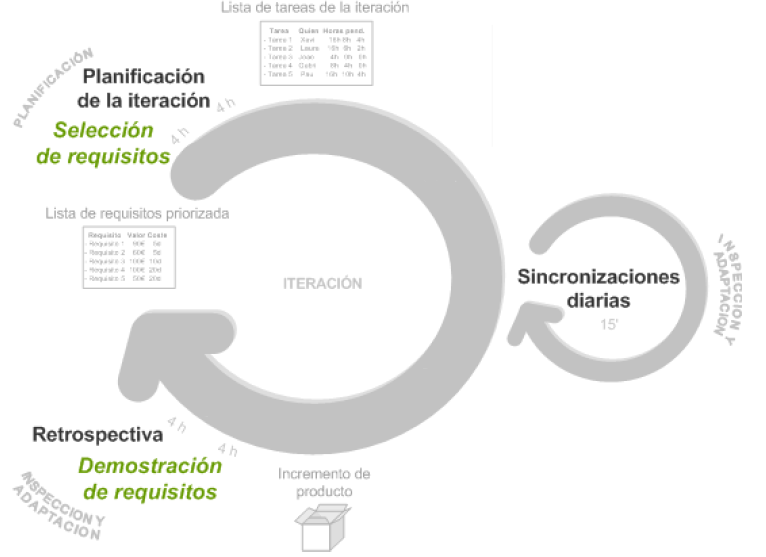
\includegraphics[width=.8\textwidth]{figures/scrum}
        \end{center}
        \caption{Esquema de trabajo de SCRUM}
        \label{scrum-esquema}
    \end{figure}
    
        \subsection{Sprint}
        
        Unidad mínima de desarrollo, usualmente determinada por una tarea corta o un período de tiempo pequeño, usualmente 1 ó 2 semanas, nunca más de 30 días; durante el cual el equipo de desarrollo trabaja según las metas estipuladas al principio del mismo. Normalmente éstas metas no cambian durante el desarrollo del Sprint sino al final del mismo, cuando se planifica el siguiente Sprint.
        
        Para HxPlus Ocupacional fue determinado en una semana para las primeras tareas y dos para las últimas, debido a las pruebas subyacentes y el trabajo de integración que representan.
        
        Se llevó a cabo 3 fases:
        \begin{enumerate}
            \item Preparación
            \item Implementación
            \item Cierre
        \end{enumerate}
        
        Tal y como se describe en el capítulo \ref{desarrollo-capitulo}.
        
        \subsection{Sprint Planning}
        
        Planificación del siguiente Sprint a realizar. El equipo de desarrollo (``Development Team", punto \ref{development-team}) hace los pronósticos e indica qué puede llevar a cabo en el siguiente Sprint de lo que propone el dueño del producto (``Product Owner", punto \ref{product-owner}) que debe hacerse durante el Sprint. El ``Scrum Master" (punto \ref{scrum-master}) está encargado de revisar cuidadosamente con el equipo las posibilidades, negociar con el dueño del producto las posibilidades de realización y establecer las metas.
        
        Semanalmente se realizó una reunión del \textit{Development Team} con el \textit{Scrum Master} y \textit{Product Owner} para evaluar el resultado del Sprint de esa semana y realizar la planificación adecuada a los logros y el desenvolvimiento en el proyecto.
        
        \subsection{Daily Sprint Meeting}
        
        Reuniones diarias realizadas entre el ``Scrum Master" y el equipo de desarrollo para revisar los avances diarios, aclarar dudas y difundir información acerca del progreso alcanzado hasta el momento. Tiempo fijo en 15 minutos y usualmente se realizan en la mañana.
        
        En este punto, Scrum, hace una diferenciación clave entre los elementos que están compromentidos (\textit{``commited"}) y los que sólo están involucrados (\textit{``involved"}) en el desarrollo del proyecto. Siendo comprometidos los equipos de desarrollo, el ``Scrum Master" y el ``Product Owner" e involucrados los demás departamentos de la empresa que puedan tener interés en el estado del proyecto (dpto. de ventas, clientes, etc). 
        
        En este órden de ideas, durante una reunión diaria de Sprint, sólo los comprometidos tienen potestad de hablar o comentar las cosas que han sucedido. Esto se hace para lograr que, en los 15 minutos de duración de la reunión, se discutan temas que sean de suma necesidad para el desarrollo del proyecto, se ponen de manifiesto dificultades técnicas o impedimentos dentro de los equipos de desarollo y, también, para difundir información sobre el estado del proyecto a las partes involucradas.
        
        La responsabilidad de resolver todo impedimento manifestado en dichas reuniones recae sobre el ``Scrum Master".
        
        Durante el proyecto se realizaron las reuniones con la presencia del Ing. Juan Jesús Albarrán para actualizar el estado del desarrollo del proyecto y aclaración de dudas por parte del pasante en cuanto a lo acaecido durante el día previo.
        
        \subsection{Sprint Review}
        
        Son reuniones que se realizan, como su nombre lo indica, para hacer una revisión del trabajo realizado durante el Sprint y presentar el trabajo completado a las partes involucradas. Estas reuniones no deben pasar de 4 horas de duración y todo trabajo incompleto no debe ser presentado.
        
        Una vez mostrados los resultados del Sprint, el ``Product Owner" debe realizar una evaluación de las metas cumplidas (o no) y si ha habido cambios en el contexto, deberá también realizar las adaptaciones necesarias a la planificación del proyecto.
        
        En \textit{HxPlus Ocupacional} se realizaoron en conjunto las reuniones de \textit{Sprint Planning} y \textit{Sprint Review} del último Sprint finalizado con la finalidad de minimizar el tiempo de reuniones y aprovechar las disponibilidades de los comprometidos y los involucrados.
        
        \subsection{Sprint Retrospective}
        
        Al finalizar cada Sprint el equipo se reúne con un tiempo fijo de 4 horas para revisar sus técnicas y la forma en que han abordado el desarrollo del proyecto, discutir las impresiones referentes al Sprint superado y revisar los inconvenientes presentados.
        
        Es deber del ``Scrum Manager" revisar los inconvenientes y buscarles solución rápida para mejorar la productividad del equipo.
        
        Debido al que el grupo de trabajo sólo consta de 1 desarrollador, se consideró inconveniente realizar reuniones de 4 horas exclusivamente para hacer la restrospectiva. En su lugar se atendieron los inconvenientes, dudas y revisones durante las reuniones diarias y se apartó un espacio de 15 minutos de las reuniones de planificación y revisión para realizar actividades de esta reunión.
        
    \section{Artefactos}
    
    Documentos realizados para llevar registro de las etapas de desarrollo del proyecto y a su vez realizar la evaluación de las mismas.
    
        \subsection{Product Backlog}
        
        O también ``Lista de Producto". Es una lista con todas las consideraciones necesarias de parte del dueño del producto, quien la organiza y la gestiona. Cualquier cambio a realizarse dentro de la planificación debe pasar por esta lista.
        
        En esta lista se enumeran los deseos del cliente, se priorizan y se estima el esfuerzo requerido. Esta lista debe ser seguida por el equipo de desarrollo para dirigir sus avances.
        
        Es una lista que hace el Dueño del Pruducto iniciando el proceso de gestión de requerimientos, sin embargo, esta lista tiene la característica de ser mutable, como los requerimientos del Dueño del Producto, y es modificada conforme sea necesario o requerido. Por eso es que \citeauthor{scrum-guia}\cite{scrum-guia} dice: ``Una Lista de Producto nunca está completa".
        
        Para ello existe el ``refinamiento" de la lista del  producto, el cual  es el proceso de añadir detalles, granularidad y prioridad a cada uno de los requerimientos, según \citeauthor{scrum-guia}\cite{scrum-guia}. Usualmente, las tareas o requerimientos que pasan a ser parte de la siguiente planificación de Sprint son las de mayor prioridad y granularidad y que, además, suele ser el caso que las actividades prioritarias son refinadas primero para así llevarlas a desarrollo lo antes posible.
        
        En el caso de \textit{HxPlus Ocupacional} el Dueño del producto realizó un levantamiento de requerimientos y utilizó ``Trello" para la gestión de los requerimientos.
    
        \subsection{Sprint Backlog}
        
        O ``Lista de Pendientes del Sprint". Es una lista de objetivos del Sprint tomada de la lista de producto durante la planificación del Sprint. Puede ser uno o varios objetivos, lo suficientemente refinados como para que el equipo de desarrollo pueda entenderlos en la reunión diaria y puedan ser llevados a cabo durante el Sprint.
        
        Según se requiera nuevo trabajo, el equipo de desarrollo lo irá añadiendo a la lista de pendientes del Sprint, ya sea por inconvenientes surgidos o problemas no tomados en cuenta o por refinamiento de los objetivos. Además, conforme el trabajo vaya siendo completado, se debe actualizar la estimación del trabajo restante. Sólo el equipo de desarrollo tiene potestad sobre la lista de pendientes del Sprint y es su forma de ver, transparentemente y en tiempo real, el estado del dearrollo de un Sprint.
        
        Usando también las facilidades de ``Trello", el equipo de desarrollo gestionó cada Sprint a través de las listas creadas dentro de una ``Pizarra" del sistema.
    
\pagebreak